%!TEX root = main.tex
%%%%%%%%%%%%%%%%%%%%%%%%%%%%%%%%%%%%%%%%%%%%%%%%%%%%%%%%%%%%%%%%%%%%%%%%%%%%%%%%

\section{Results}
\label{sec:results}

\begin{figure}[t]
\centering
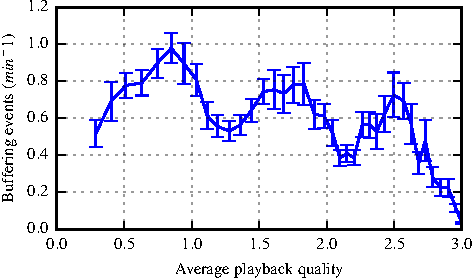
\includegraphics[width=0.95\linewidth]{figs/33qualityvstalling}%
\caption{Average playback quality versus stalling events}
\label{fig:qualityvsstalling}%
\end{figure}

Figure \ref{fig:qualityvsstalling} illustrates the relationship between the average quality level and the stalling events in the experiment result set.
For the average quality level, 0 is defined as \unit[100]{\%} of the segments are shown to the user in 144p. 3 is defined as \unit[100]{\%} of the segments are shown to the user in 480p.
The average quality levels are clustered using k-means and the error bars indicate the \unit[95]{\%} confidence interval of each cluster.
Two observations can be made from the figure. 
First, the lowest average quality level is 0.3 with about 0.5 switches per minute.
From this it follows that the player risks one stalling per two minutes in order to avoid showing only the lowest quality level in low bandwidth scenarios.
Second, the buffering events exhibit an oscillating behavior.
The oscillating behavior is consistent with observations made in \cite{sieber16sacrificing}.
The study shows that the performance of YouTube's adaptation algorithm depends on the ratio between video bit-rate and available bandwidth.
For certain ratios, the algorithm is able to efficiency use available bandwidth, i.e. there is only a low amount of redundant traffic and buffering.
Other ratios exhibit a high amount of redundant traffic and buffering ratio.
%There exists a fixed ratio of about three times the bit-rate compared to the network throughput (i.e. not application level throughput), where the time on that quality level is maximized, but also the quality switching and buffering ratio is increased.

In total, the pearson correlation shows a high correlation (-0.774) between average quality level and buffering events.
\subsection{Data Sets}

Idea: calculate the highest resolution that could have been achieved. compare it to measurement data. How much can still be gained?
In the following we want to compare three optimization methods to each other.
opt was calculated according to the optimization problem in \cite{hossfeld2015identifying}. The calculations were done using the Gurobi Optimizer\footnote{http://www.gurobi.com/}.

In total we have four sets of results that we compare to each other:
First, we have the initial observations which shall serve as a \textit{baseline} in the following analysis. Please notice that stalling events did occur during these runs. These measurements were originally recorded in \cite{sieber16sacrificing} where the measurement methodology and measurement set-up is described in great detail: $35$ videos $\times 27$ bandwidth values $\times 15$ replications. Four quality level representations were observed: $144p, 240p, 360p, 480p$.

Based on this dataset, a \textit{heuristical approach} was calculated in \cite{sieber16sacrificing} which estimated the average resolution that is reachable if there was no redundant traffic, i.e. if no video segment is downloaded multiple times. Notice that it was assumed that the same amount of stalling would occur.

As a new contribution, we use the optimization problem, described in \ref{fig:opt} to exactly calculate the highest mean resolution that was optimally obtainable. Hereby, we consider the same video files, the same duration of the viewing session and the same average network throughput as was used in the baseline scenario to make it comparable. However, instead of having stalling events interrupt the replaying process, we added an initial delay to the the replaying process. The duration of this delay is equal to the sum of the observed stalling events. This leads to the same duration of the viewing session and the same replay time and the same amount of data that was totally downloaded.

Our second approach was to eliminate the stalling completely and reduce the initial delay to the minimum possible duration. For this, we considered the exact same network throughput as in the baseline scenario, while having a shorter session duration since the stalling times are omitted. This means that the amount of data that is downloaded in this case is lower than in the baseline scenario.

More details for \textit{opt (no stalling, no initial delay)}
\begin{itemize}
\item optimization done according to 2-step approach from \cite{miller2013optimal}
\item we assume no initial delay
\item this means, the total duration of a video session is lower if stalling occured in the measurement run. This means less total data is downloaded.
\end{itemize}
\textit{opt (initial delay instead of stalling)} was done similar to \textit{opt no stalling} with the difference that we added an initial delay $T_0$ to the replaying process. The duration of $T_0$ was equal to the total duration of all stalling events combined. This way, it is ensured that the same amount of data can be downloaded.

\subsection{Optimal Adaptation}

First, we will look at the adaptation of video resolution; second we will look at how many switches are expected to occur.

\begin{figure}[t]
\centering
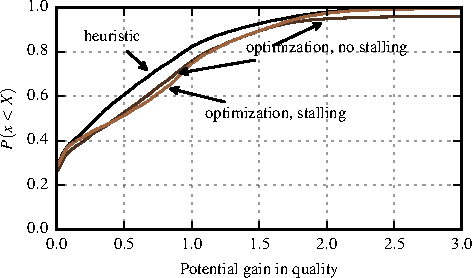
\includegraphics[width=0.5\textwidth]{figs/qualitygain_py}%
\caption{CDF of the mean video quality in the measurement runs and highest achievable mean video quality according to the optimization problem in \cite{hossfeld2015identifying}. Remake figure!}
\label{fig:opt}%
\end{figure}

\begin{figure}[t]
\centering
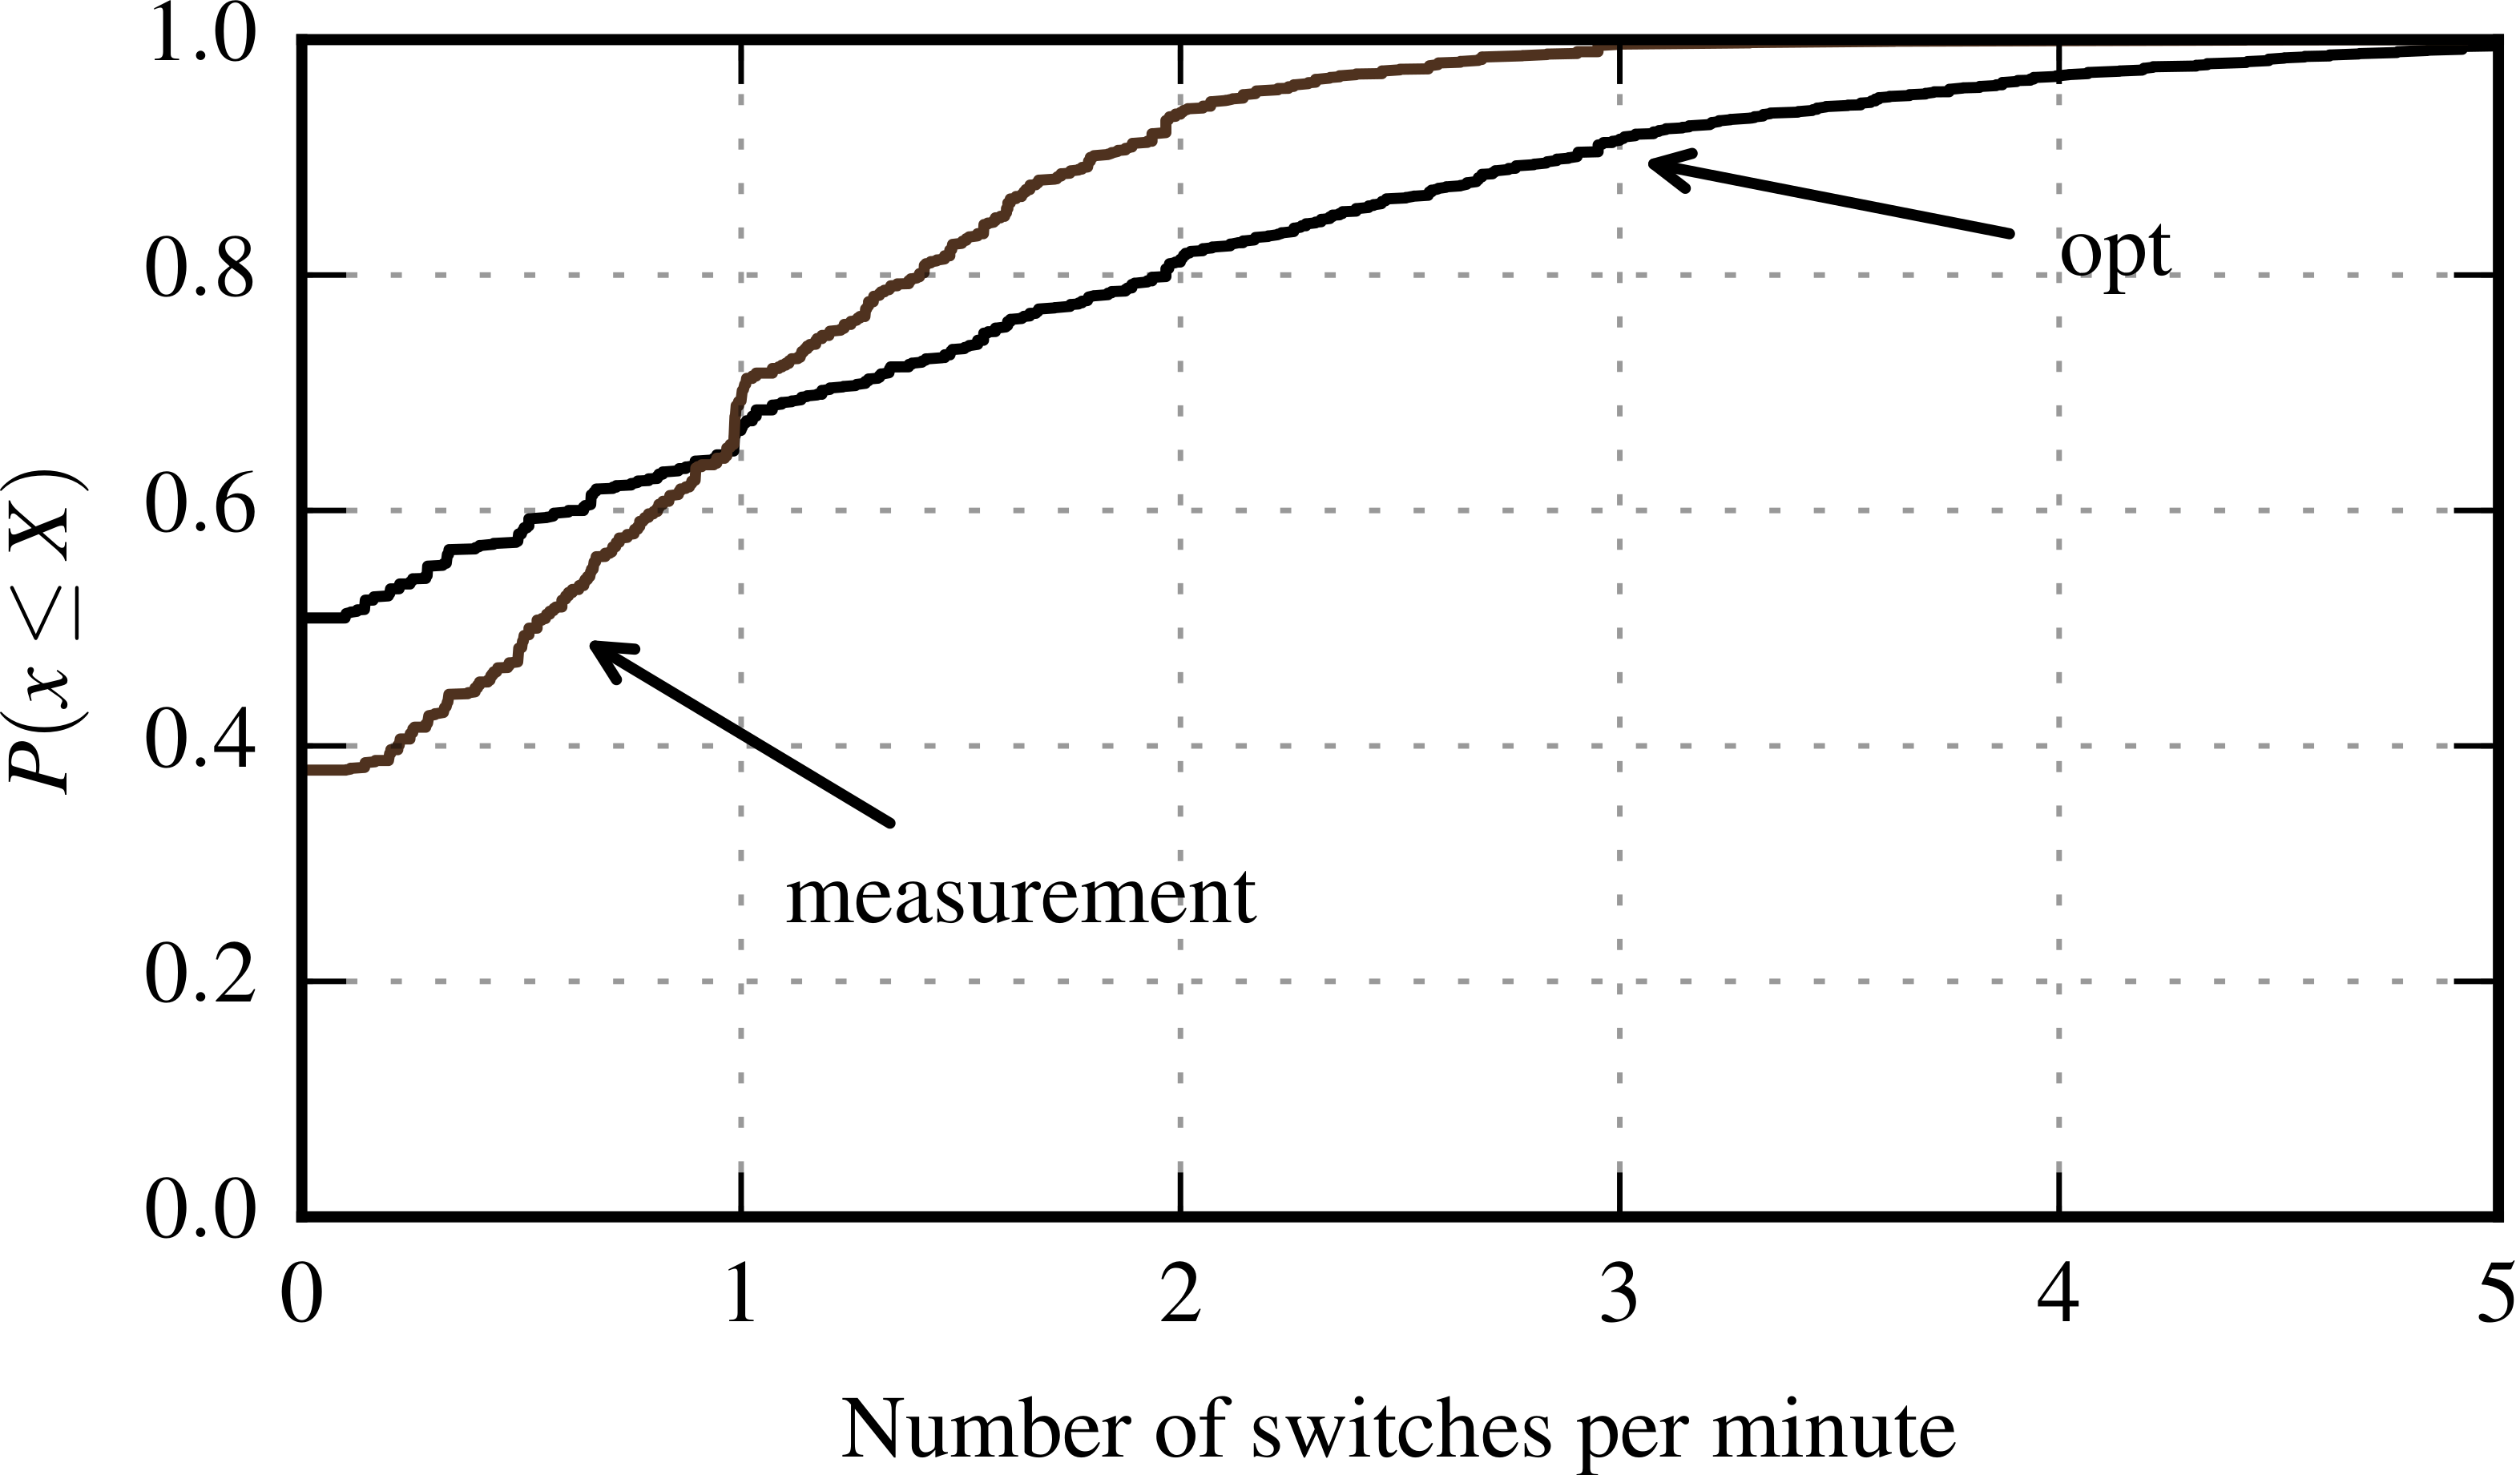
\includegraphics[width=0.5\textwidth]{figs/switches_py}%
\caption{CDF of the number of switches per minute. Remake figure!}
\label{fig:switches}%
\end{figure}

In figure \ref{fig:opt} we see the CDF of the mean video quality in the measurement runs and highest achievable mean video quality according to the optimization problem. In addition, we added an estimation of the avg. quality level that is possible based on downloaded data that was done in \cite{sieber16sacrificing}. While stalling events occured frequently during the original measurement, stalling events are not allowed to occur in the optimization problem. Therefore, we consider two sets of input for the opt. prob. for each measurement run: First, we only consider the available bandwidth during the video download. Second, we also respect the stalling events that occured. The sum of stalling was then added as initial delay during which the video was downloaded. In contrast to the YouTube measurement data where the video buffer does not contain more than 50s of video content at a time, in the calculations of the optimal adaptation we assumed that the video buffer is not limited.
